\documentclass[a4paper]{article}

\usepackage{pdp}

%------------------------------------------------------------------------------
%	REPORT INFORMATION
%------------------------------------------------------------------------------

\title{Quoridor -- Java}
\subtitle{Rapport final}
\author{Abdeldjabar Ismail Abdraman, Cengiz Vasseur, Joris Douillet, Khadidja Ahmat Hassan, Matthieu Pourageaud}

%------------------------------------------------------------------------------

\begin{document}

%------------------------------------------------------------------------------
%	TITLE P
%------------------------------------------------------------------------------

\maketitle
\thispagestyle{empty}

%------------------------------------------------------------------------------
%	MAIN MATTER
%------------------------------------------------------------------------------

\section{Les Fonctionnalités étendues}

\subsection{Fonctionnalité 1 : Réseau client/serveur et gestion multi-clients}

\subsubsection{Besoin initial}
L’un des objectifs du projet était d’ajouter une dimension réseau au jeu Quoridor afin de permettre à plusieurs joueurs d’interagir à distance. Dans une première étape, il s’agissait de mettre en place un serveur simple capable d’accepter une connexion cliente, de répondre à des commandes élémentaires telles que \texttt{PING} et \texttt{QUIT}, et de permettre au client de tester la connexion.

Dans une seconde étape, l’objectif a été étendu à la gestion simultanée de plusieurs clients et de plusieurs parties en parallèle. Le serveur devait alors être capable de conserver l’état de plusieurs sessions de jeu, de créer des parties entre joueurs disponibles, de valider les coups reçus à distance et de transmettre les actions aux autres joueurs concernés.

L’intérêt de cette fonctionnalité est double. D’une part, elle transforme le jeu local en application distribuée selon une architecture client/serveur. D’autre part, elle centralise la validation des coups côté serveur, ce qui évite qu’un client applique localement des actions non vérifiées.

\subsubsection{Choix de conception}
Le choix retenu dans le projet est une architecture client/serveur. Le serveur joue le rôle d’autorité centrale : il accepte les connexions, reçoit les commandes, valide les actions envoyées par les clients et conserve l’état officiel des parties.

L’implémentation repose sur deux niveaux principaux. La classe \texttt{GameServer} correspond à un serveur simple, conçu pour la première étape du réseau. Elle gère une seule connexion cliente, répond à des commandes de base comme \texttt{PING} et \texttt{QUIT}, lance un diffuseur UDP et met en place un timeout d’une minute. La classe \texttt{MultiGameServer} constitue l’extension multi-clients.

Le protocole choisi est volontairement simple : les messages échangés sont des chaînes ASCII terminées par un retour à la ligne. Les commandes principales sont \texttt{HELLO}, \texttt{PING}, \texttt{QUIT} et \texttt{MOVE}, avec des réponses comme \texttt{WELCOME}, \texttt{PONG}, \texttt{BYE}, \texttt{OK}, \texttt{ERROR}, \texttt{GAME\_START}, \texttt{OPPONENT\_MOVE} et \texttt{GAME\_OVER}.

Pour l’annonce de présence du serveur, le projet utilise une classe \texttt{ServerBroadcaster}. Côté client, la méthode \texttt{serverList()} de \texttt{GameClient} écoute les messages UDP afin de détecter les serveurs disponibles.

Enfin, la validation des coups ne repose pas sur le client. Lorsqu’un joueur envoie un coup sous forme textuelle, celui-ci est converti en objet métier \texttt{Move} par \texttt{NetworkMoveParser}, puis transmis au moteur de jeu côté serveur.

\subsubsection{Structures de données utilisées}
La partie réseau s’appuie sur plusieurs structures de données importantes.

Dans \texttt{MultiGameServer}, les clients sont stockés dans une structure \texttt{Map<String, ClientSession>}. Chaque client possède un identifiant unique (C1, C2, etc.).

Les parties actives sont stockées dans \texttt{Map<String, ServerGameSession>}.

Le tableau des scores repose sur \texttt{Map<String, ScoreEntry>}.

La synchronisation repose sur un verrou utilisé avec \texttt{synchronized(lock)}.

Côté client, \texttt{GameClient} utilise une \texttt{SynchronousQueue<String>} pour gérer les réponses synchrones.

\subsubsection{Algorithme mis en place}
Le serveur ouvre une socket TCP, lance un thread UDP pour la diffusion et un thread de surveillance pour les timeouts.

Chaque connexion crée une \texttt{ClientSession}. Lorsqu’un client envoie une commande :
\begin{itemize}
    \item \texttt{HELLO} : enregistre le joueur
    \item \texttt{PING} : réponse \texttt{PONG}
    \item \texttt{QUIT} : réponse \texttt{BYE}
    \item \texttt{MOVE} : traitement du coup
\end{itemize}

Pour un coup :
\begin{itemize}
    \item Vérification du joueur et du tour
    \item Conversion en \texttt{Move}
    \item Validation par le moteur de jeu
\end{itemize}

Si le coup est valide :
\begin{itemize}
    \item Envoi de \texttt{OK}
    \item Diffusion de \texttt{OPPONENT\_MOVE}
\end{itemize}

Fin de partie :
\begin{itemize}
    \item Mise à jour du score
    \item Envoi de \texttt{GAME\_OVER WIN} ou \texttt{GAME\_OVER LOSE}
\end{itemize}

\subsubsection{Difficultés rencontrées}

La principale difficulté de cette fonctionnalité a été la gestion de la concurrence. En effet, dans la version multi-clients, le serveur fonctionne avec plusieurs threads
: un thread principal d’acceptation des connexions, un thread par client, un thread pour le diffuseur UDP et un thread pour la surveillance des timeouts. Sans mécanisme de protection,
plusieurs accès simultanés aux listes de clients, de parties ou de scores auraient pu provoquer des incohérences. L’utilisation d’un verrou commun avec synchronized (lock) a donc été nécessaire.

Une deuxième difficulté a concerné la gestion des réponses synchrones et des messages asynchrones côté client.
Certaines commandes, comme PING ou QUIT, attendent une réponse précise et immédiate. En parallèle,
d’autres messages peuvent arriver à tout moment depuis le serveur, par exemple WELCOME, OPPONENT\_MOVE ou GAME\_OVER.
Il a donc fallu concevoir un client capable de lire les messages en continu tout en permettant à certaines méthodes d’attendre
une réponse particulière. Cette difficulté a été traitée dans GameClient avec un thread d’écoute et une file de synchronisation.

Une troisième difficulté a été l’intégration du protocole réseau avec la logique métier du jeu.
Le serveur ne se contente pas de relayer les messages ; il doit interpréter un coup reçu sous forme textuelle,
le convertir correctement en objet métier et vérifier sa légalité avec le moteur du jeu.
Cela impose une bonne articulation entre les classes réseau et les classes du noyau du projet.

Enfin, la découverte de serveurs a demandé une conception séparant deux types d’échanges :
le TCP, utilisé pour la communication fiable entre client et serveur pendant la partie, et l’UDP, utilisé pour l’annonce de présence du serveur.
Dans l’état actuel du projet, cette partie existe bien mais reste encore partiellement finalisée.


\subsubsection{Tests réalisés}

La fonctionnalité réseau a été accompagnée de plusieurs tests unitaires.

La classe GameServerTest vérifie le fonctionnement du serveur simple. Les tests confirment qu’un client peut se connecter, qu’un message PING reçoit bien PONG, qu’une commande QUIT reçoit BYE, et qu’une commande inconnue reçoit une réponse générique.

La classe GameClientTest vérifie les comportements essentiels du client. Les tests contrôlent la réussite ou l’échec d’une connexion, l’affichage d’un message d’erreur lorsqu’aucune connexion n’est active, l’envoi correct des commandes HELLO, MOVE et QUIT, ainsi que la commande serverList() à l’aide d’un faux serveur UDP.

La classe MultiGameServerTest couvre une partie importante de la logique multi-clients. On y retrouve notamment des tests sur l’état du serveur, la liste des joueurs, le tableau des scores, la création de parties à deux ou quatre joueurs, le changement de statut des joueurs, la gestion des tours, les erreurs liées à un joueur absent ou indisponible, ainsi que certains comportements liés à la validation des coups, à leur diffusion et à la fin d’une partie.

D’autres tests existent également autour de classes connexes comme NetworkMoveParserTest, ServerBroadcasterTest, ClientSessionTest, ServerGameSessionTest et NetworkLauncherTest. Dans l’ensemble, ces tests montrent que la partie réseau n’a pas seulement été commencée, mais qu’elle a réellement été structurée et vérifiée

Les tests couvrent :
\begin{itemize}
    \item \texttt{GameServerTest} : tests du serveur simple
    \item \texttt{GameClientTest} : tests du client
    \item \texttt{MultiGameServerTest} : tests multi-clients
\end{itemize}

D’autres tests existent : \texttt{NetworkMoveParserTest}, \texttt{ServerBroadcasterTest}, etc.

\subsubsection{Résultat final}
La fonctionnalité réseau est globalement fonctionnelle. Le serveur multi-clients permet de gérer plusieurs joueurs, parties et scores.

Cependant, certains points restent à améliorer, notamment la découverte complète des serveurs et l’intégration totale dans toutes les interfaces.



\section{Architecture du projet}

\subsection{Justification du choix d’architecture}

Comme décrit dans le cahier des charges, notre projet qui consiste a implementer le jeu quoridor en java
decrit au ci-haut doit respecter l’ensemble des règles du jeu Quoridor.
De plus, il nous est demandé de mettre en œuvre trois modes d’interaction :
ligne de commande (CLI), interface graphique (GUI) et jeu en réseau, ainsi
que plusieurs intelligences artificielles (Minimax et Monte Carlo Tree Search).


Pour répondre à tous ces exigences, nous avons opté pour une architecture modulaire orientée domaine,
inspirée de la Clean Architecture\cite{martin2017clean}.

La Clean Architecture repose sur un principe fondamental : la séparation entre la logique métier et les détails d’implémentation. Dans ce modèle :
Le cœur domaine contient toutes les entités métier de l’application. Il est totalement indépendant.
Les adaptateurs  (CLI, GUI, réseau, persistance, IA) interagissent avec le cœur via des interfaces abstraites et des implémentations concrètes.
par cette architecture nous garantisons  la cohérente du logique métier, on peut  facilement ecrire des teste,
ajouter de nouvelles IA ou interfaces et nous sommes sur de la robustesse de notre jeu, car toutes les actions passent par la validation du cœur métier et en fin on peut facilement
Maintenir notre jeu, car les modifications sur l’interface n’impactent pas le cœur.


\subsection{Vue d'ensemble des packages}

Voici les  onze packages distincts de notre projet, chacun ayant une responsabilité bien définie que les decrivons de
manieres brefs ici:


\begin{table}[H]
\centering
\begin{tabular}{|p{2cm}|p{13cm}|}
    \hline
    \textbf{Package} & \textbf{Responsabilité} \\
    \hline
    core & Entités métier : Board, GameState, Player, Move, Position, GameEngine, RuleChecker \\
    \hline
    Main & Point d'entrée, résolution du mode de lancement, patron Factory \\
    \hline
    cli & Interface en ligne de commande avec le pattern Command pour chaque action utilisateur \\
    \hline
    gui & Interface graphique comportant les menus 'File' et 'Game' (JavaFX), proposant des raccourcis clavier. L’utilisateur doit pouvoir définir ses propres raccourcis pour chaque action listée \\
    \hline
    network & Implémente les commandes réseau de base et étendues pour gérer plusieurs clients simultanément, en utilisant un thread par client ou de la programmation asynchrone. Serveur TCP avec découverte UDP et client réseau \\
    \hline
    ai & Joueurs IA : Random, Minimax (alpha-beta, iterative deepening), MCTS, réseau de neurones \\
    \hline
    persistence & Sérialisation/désérialisation de l’état de jeu vers un fichier texte \\
    \hline
    util & Logger singleton partagé dans toute l’application \\
    \hline
    i18n & Gestion de la langue du logiciel. Si les variables d’environnement 'LANG' ou 'LC\_ALL' sont définies, le programme doit les utiliser pour déterminer la langue à utiliser \\
    \hline
    graph & Module Graph et GraphBuilder implémenté sous la forme d’une liste d’adjacence (adjacency list) pour représenter l’état du plateau de jeu \\
    \hline
    config & Fichier de configuration nommé '.quoridorrc', placé à la racine du répertoire de l’utilisateur (HOME). Le fichier est lu au démarrage du programme s’il est présent, et les options qu’il contient sont utilisées par défaut. Sinon, un fichier de configuration minimal est créé automatiquement \\
    \hline
\end{tabular}
\caption{Vue d'ensemble des packages}
\label{tab:packages}
\end{table}

\subsection{Vue en couches concentriques}
Dans cette section nous vous proposons notre archichesture global en couches concentriques.
les dependances entre packages ne doivent pointer que vers l'interieur du systeme. Le
module \textbf{core} qui contient les entites metier — ne connait aucun autre
module. C'est \textbf{network}, \textbf{gui} ou \textbf{cli} qui dependent de \textbf{core},
jamais l'inverse. Cette contrainte est visible dans le diagramme.

schema en couches concentriques de notre architecture du projet (Fig.~\ref{fig:example1}).
\begin{figure}[H]
    \centering
    \frame{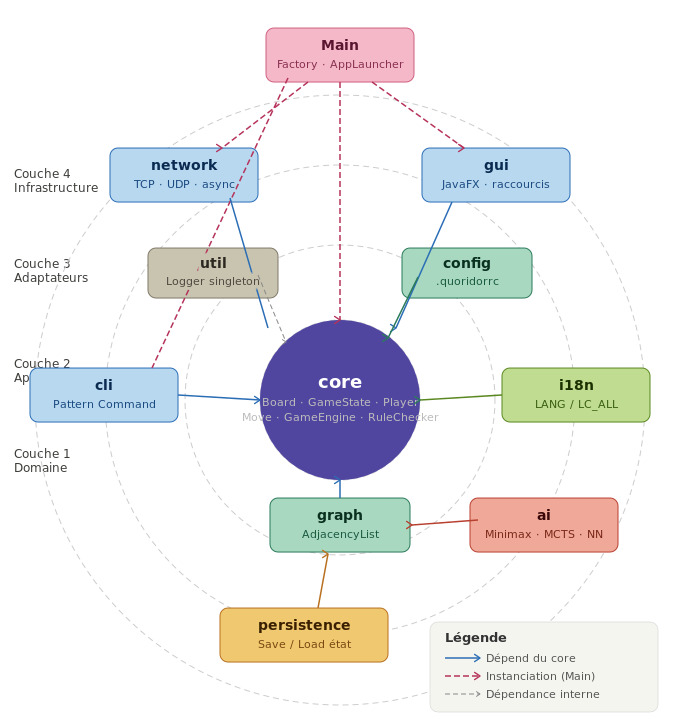
\includegraphics[width=.85\textwidth]{architecture_quoridor.jpg}}
    \caption{Une architecture en couches}\label{fig:example1}
\end{figure}

\subsection{Couche Domaine --- Package \texttt{core}}


Le module \textbf{core} est le coeur du systeme. Il encapsule l'integralite de la logique
metier du jeu et n'a aucune dependance externe. Le \textbf{RuleChecker}
appelle le module \textbf{graph} pour verifier qu'apres la pose d'un mur, chaque joueur dispose encore
d'un chemin vers son bord cible.

voici un diagramme indique comment son lié les differents classes du package core.

schema du couche core de notre architecture(Fig.~\ref{fig:example0}).
\begin{figure}[H]
    \centering
    \frame{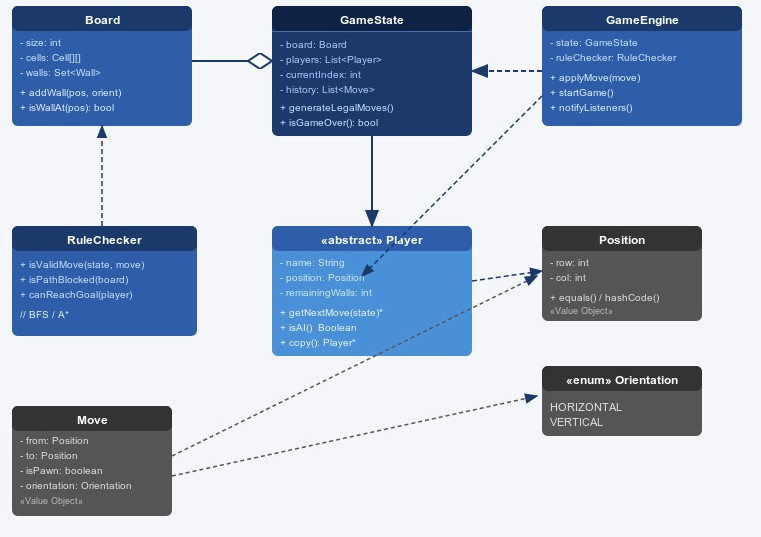
\includegraphics[width=.65\textwidth]{core.jpg}}
    \caption{Une architecture en couches}\label{fig:example0}
\end{figure}

\subsection{Couche Principale --- Package \texttt{Main}}
Le module \textbf{Main} joue le role de \textbf{composition root}
: il instancie tous les autres modules et cable leurs dependances. Il utilise le pattern \textbf{Factory}
via \textit{AppLauncher} pour creer les adaptateurs selon le mode de lancement.

Au demarrage, le Main lit config (.quoridorrc) pour determiner le mode de jeu. Il instancie network si une partie reseau est demandee, gui pour le
mode graphique, cli pour le mode terminal. Il injecte les dependances dans chaque module sans que ceux-ci se connaissent mutuellement.

voici un diagramme indique comment son lié les differents classes du package main.

schema du couche main de notre architecture (Fig.~\ref{fig:example2}).
\begin{figure}[H]
    \centering
    \frame{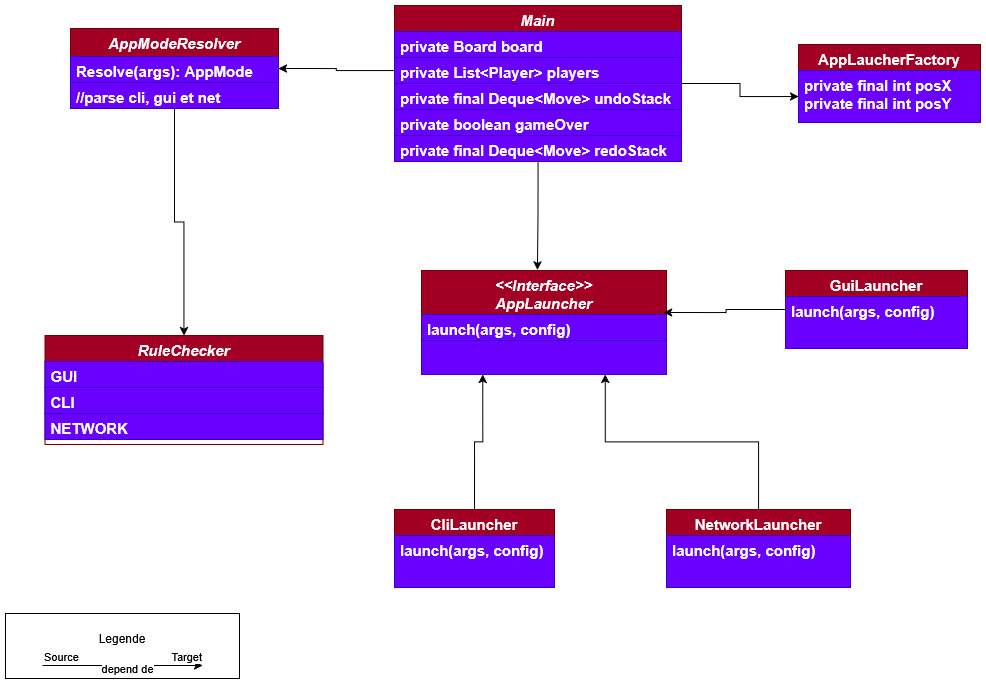
\includegraphics[width=.65\textwidth]{main}}
    \caption{Une architecture en couches}\label{fig:example2}
\end{figure}

\subsection{Interface CLI --- Pattern Command}
Le  module \textbf{cli} implemente le pattern \textbf{Command}
: chaque commande saisie est encapsulee dans un objet qui connait son
action et peut etre annulee. Ce pattern est adapte a Quoridor car il
permet de rejouer ou d'annuler l'historique des coups. Notre  cli  est instancie par Main au meme titre que gui et network. Il lit les
entrees console, les parse, construit les objets Command correspondants et les execute sur \textit{GameEngine}.
Le plateau est affiche en ASCII en sortie standard.

voici un diagramme indique comment son lié les differents classes du package cli.


schema du couche cli de notre architecture (Fig.~\ref{fig:example3}).
\begin{figure}[H]
    \centering
    \frame{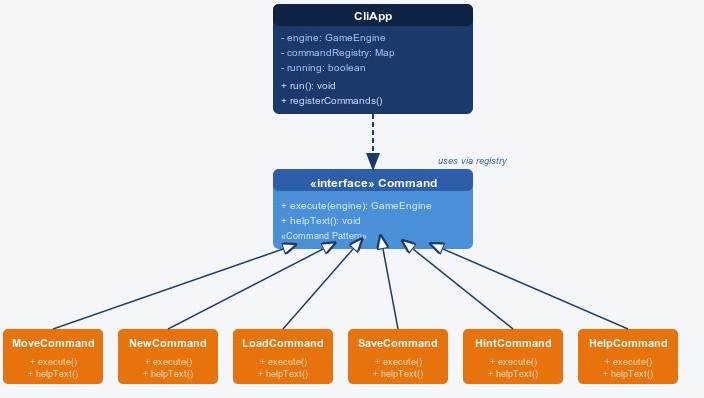
\includegraphics[width=.65\textwidth]{cli}}
    \caption{Une architecture en couches}\label{fig:example3}
\end{figure}


\subsection{Points forts architecturaux}

\begin{itemize}
  \item \textbf{Indépendance du domaine} : le package \texttt{core} est du Java pur, sans dépendance externe
  \item \textbf{Extensibilité de l’IA} : tout nouvel algorithme étend simplement \texttt{AiPlayer}
  \item \textbf{Pattern Command en CLI} : chaque commande est testable et extensible indépendamment
  \item \textbf{Persistance découplée} : \texttt{GameSaver} / \texttt{GameLoader} ne connaissent que les interfaces du \texttt{core}
  \item \textbf{Builder pour MinimaxPlayer} : configuration déclarative et lisible de l’IA
\end{itemize}

\subsection{Axes d'amélioration}




%------------------------------------------------------------------------------
%	BIBLIOGRAPHY
%------------------------------------------------------------------------------

\nocite{*}
\bibliographystyle{plain}
\bibliography{bibliography}

%------------------------------------------------------------------------------
% BACK MATTER
%------------------------------------------------------------------------------
\appendix

\section{Section en annexe}

\begin{table}[H]
    \centering
    \begin{tabular}{|p{1.5cm}|p{3cm}|p{8.5cm}|p{2cm}|}
        \hline
        \textbf{Besoins} & \textbf{Titre du besoin} & \textbf{Description du besoin} & \textbf{État} \\
        \hline
        F1 & Lancement & Lancement via CLI avec options (-h, -V, -v, -d) et gestion des flux stdout/stderr. & FAIT \\
        \hline
        F2 & Configuration & Lecture et création du fichier .qoridorrc au format INI dans le HOME. & FAIT \\
        \hline
        F3 & i18n & Support de l'anglais et du français via les variables LANG/LC\_ALL. & FAIT \\
        \hline
        F4 & Interface CLI & Démarrage auto, application des options ou chargement d'une sauvegarde. & FAIT \\
        \hline
        F5 & Mode Blitz & Mode avec temps limité par joueur (-b) et réglage de la durée (-t). & FAIT \\
        \hline
        F6 & Mode Contest & Lecture d'un fichier de position et réponse du meilleur coup sur stdout. & FAIT \\
        \hline
        F7 & Interface Graphique & Lancement d'une fenêtre GUI via l'option -g ou --gui. & FAIT \\
        \hline
        F8 & Mode IA & Remplacement d'un ou plusieurs joueurs par une intelligence artificielle. & FAIT \\
        \hline
        F9 & Options Spécifiques & Paramétrage du nombre de joueurs (2-4), des murs et de la taille du plateau (3-15). & FAIT \\
        \hline
        F10 & Gestion des règles & Arbitrage du jeu, validation des coups, calcul des scores et victoire. & FAIT \\
        \hline
        F11 & Erreurs Utilisateur & Gestion robuste des mauvaises saisies avec messages explicites. & FAIT \\
        \hline
        F12 & Undo/Redo & Historique des coups et possibilité d'annuler/rétablir pour les humains. & FAIT \\
        \hline
        F13 & Conseils & Système d'aide suggérant le meilleur coup à jouer selon l'état actuel. & FAIT \\
        \hline
        F14 & Gestion Blitz & Affichage du chronomètre, gestion de la pause et défaite au temps. & FAIT \\
        \hline
        F15 & Shell interactif & CLI sous forme de shell avec commandes (new, save, load, show, etc.). & FAIT \\
        \hline
        F16 & Sauvegarde/Quitter & Confirmation de sauvegarde lors de la fermeture si la partie est modifiée. & FAIT \\
        \hline
        F17 & Édition ligne & Support de l'édition de ligne (curseur) via Readline ou équivalent. & FAIT \\
        \hline
        F18 & Historique Shell & Navigation dans les anciennes commandes et recherche par le caractère "+". & FAIT \\
        \hline
        F19 & Complétion & Autocomplétion des commandes via la touche Tabulation. & FAIT \\
        \hline
    \end{tabular}
    \caption{Vue d'ensemble des besoins et leurs realisations}
    \label{tab:besoins4colonnes0}
\end{table}

\begin{table}[H]
    \centering
    \begin{tabular}{|p{1.5cm}|p{3cm}|p{8.5cm}|p{2cm}|}
        \hline
        F20 & Notation des coups & Représentation ASCII du plateau et syntaxe de mouvement (ex: e2-e3, e2v). & FAIT \\
        \hline
        F21 & Format Sauvegarde & Import/export en format texte ASCII avec paramètres, état et historique. & FAIT \\
        \hline
        F22 & Commentaires & Support des commentaires mono-ligne (\#) et bloc (\{ \}) dans les sauvegardes. & FAIT \\
        \hline
        F23 & Paramètres Jeu & Format clé-valeur pour les réglages dans le fichier de sauvegarde. & FAIT \\
        \hline
        F24 & Format Plateau & Représentation visuelle simplifiée du plateau pour la restauration. & FAIT \\
        \hline
        F25 & Format Historique & Liste chronologique des tours et des coups par joueur. & FAIT \\
        \hline
        F26 & Module Graph & Utilisation d'une liste d'adjacence et algorithmes de graphes indépendants. & FAIT \\
        \hline
        F27 & Algos Graphes & Calcul des coups valides, scores et détection de fin de partie via le graphe. & FAIT \\
        \hline
        F28 & Menus GUI & Implémentation des menus 'File' et 'Game' dans l'interface graphique. & FAIT \\
        \hline
        F29 & Raccourcis Clavier & Raccourcis Ctrl+N, S, O, etc. et personnalisation via configuration. & FAIT \\
        \hline
        F30 & Drag'n'Drop & Manipulation des pièces et des murs à la souris dans le GUI. & FAIT \\
        \hline
        F31 & IA : Temps borné & Limite de réflexion de l'IA (5s par défaut) avec coup par défaut si dépassé. & FAIT \\
        \hline
        F32 & IA : Minimax & Implémentation de l'algorithme Minimax avec élagage Alpha-Beta. & FAIT \\
        \hline
        F33 & IA : Fonctions Score & Au moins 3 fonctions d'évaluation différentes pour l'IA Minimax. & FAIT \\
        \hline
        F34 & IA : Deepening & Mode approfondissement itératif pour optimiser la recherche. & FAIT \\
        \hline
        F35 & IA : Profondeur & Option pour fixer la profondeur max de recherche de l'algorithme. & FAIT \\
        \hline
        F36 & IA : MCTS & Algorithme Monte Carlo Tree Search avec fonction UCT. & FAIT \\
        \hline
        F37 & IA : Machine Learning & Fonction de sélection MCTS basée sur l'apprentissage automatique (ML). & FAIT \\
        \hline
        F38 & Réseau : Basique & Découverte UDP, connexion TCP, ping/pong et client/serveur simple. & FAIT \\
        \hline
        F39 & Réseau : Multi-clients & Serveur gérant plusieurs parties, scoreboard et validation anti-triche. & NON FAIT \\
        \hline
        F40 & Réseau : Invitations & Système avancé d'invitations (accept/decline) et gestion des statuts joueurs. & NON FAIT \\
        \hline
    \end{tabular}
    \caption{Vue d'ensemble des besoins leurs realisations}
    \label{tab:besoins4colonnes}
\end{table}

\end{document}
